\subsection{XGBoost}

 Table \ref{tab:xgb-scv-metrics} summarises the average metrics with 10 Fold S-CV, and Table \ref{tab:xgb-test-metrics} shows the metrics across the 30\% test set. Due to the numerous models created during experimentation, only the most notable models are included in the tables. The raw metrics for all models can be found in \ref{appx:XGBoost}. 

\begin{table}[h]
\centering
\caption{XGBoost S-CV Metrics}
\label{tab:xgb-scv-metrics}
\begin{tabular}{|l|l|l|l|l|l|l|l|}
\hline
\textbf{Model ID} & \textbf{Dataset} & \textbf{AUC} & \textbf{F1} & \textbf{Precision} & \textbf{Recall} & \textbf{Accuracy}  \\ \hline
6 & 100\% & 99.99 & 99.64 & 99.64 & 99.64 & 99.64 \\ \hline
8 & 100\% & 99.99 & 99.64 & 99.64 & 99.65 & 99.65 \\ \hline
10 & 100\% & 100.00 & 99.65 & 99.65 & 99.66 & 99.66 \\ \hline
11 & 100\% & 100.00 & 99.64 & 99.64 & 99.65 & 99.65 \\ \hline
\end{tabular}
\end{table}

\begin{table}[H]
\centering
\caption{XGBoost Test Metrics}
\label{tab:xgb-test-metrics}
\begin{tabular}{|l|l|l|l|l|l|l|l|}
\hline
\textbf{Model ID} & \textbf{Dataset} & \textbf{AUC} & \textbf{F1} & \textbf{Precision} & \textbf{Recall} & \textbf{Accuracy}  \\ \hline
0 & 60\% & 99.99 & 99.63 & 99.64 & 99.64 & 99.64 \\ \hline
1 & 80\% & 99.99 & 99.64 & 99.65 & 99.65 & 99.65 \\ \hline
2 & 80\% & 99.99 & 99.64 & 99.64 & 99.64 & 99.64 \\ \hline
3 & 80\% & 99.99 & 99.64 & 99.64 & 99.64 & 99.64 \\ \hline
5 & 80\% & 99.99 & 99.64 & 99.65 & 99.65 & 99.65 \\ \hline
6 & 100\% & 99.99 & 99.65 & 99.65 & 99.65 & 99.65 \\ \hline
8 & 100\% & 99.99 & 99.65 & 99.65 & 99.65 & 99.65 \\ \hline
10 & 100\% & 99.99 & 99.65 & 99.65 & 99.66 & 99.66 \\ \hline
11 & 100\% & 99.99 & 99.65 & 99.65 & 99.65 & 99.65 \\ \hline
\end{tabular}
\end{table}

\smallskip
Models 0, 1 and 6 were trained across varying levels of data sizes, but the models shared similar performance metrics. Model 0, trained on 60\% of the dataset, slightly underperformed in classifying minority classes as seen in the F1, precision and recall scores from the classification report. Model 1 showed a similar pattern but had a minor increase in correct classifications, especially for SSH. Model 6, being trained on more data, subsequently achieved a better result across most classes and can be seen in the classification report and confusion matrix. Precision and recall in the testing set were also increased. Although minor, the gradual improvement shows the positive impacts more data can have to help a model train and learn the patterns and complexities of the dataset, allowing it to generalise well on unseen data.

\smallskip
In Model 3, 80\% of the dataset was used, and early stopping of 10 rounds and regularisation of 0.1 was added to the model. However, analysing the metrics in detail, models 1/2 share a similar performance. Both equally have high precision and recall, and the weighted averages are very similar; the confusion matrices show minor differences but did not significantly affect performance. Adding early stopping and regularisation to model 3 did not significantly affect the model's performance compared to the baseline. 

\medskip

\subsubsection*{GridSearchCV}

\smallskip
One instance of GridSearchCV ran successfully that tested a combination of the learning rate, number of estimators and the max depth. The test was cross-validated five times and took 28.27 hours to complete. Models 5 (80\%) and 8 (100\%) were created with these parameters. The results are incomparable compared to their baseline counterparts (4 and 6). Model 5 shares identical values for AUC and F1, with a 0.1 increase in Precision, Recall and Accuracy; this is also similar in Model 8, except AUC rounds to 100. To summarise, the models with default parameters (Models 4 and 6) and those with the best-found parameters from GridSearchCV (Models 5 and 8) have similar performances across both datasets. Model 11 adopts the same parameters with the added inclusion of S-CV, early stopping and regularisation. However, there were no significant improvements with similar high metrics and behaviour.

\subsubsection*{RandomisedSearchCV}

\medskip

A parameter grid was tested with RandomisedSearchCV and took 41.81 hours to complete. Each parameter combination was subjected to 10-fold Stratified Cross Validation to measure its performance. 

A new model was created with the best-found parameters, Model 10. The model performed very well, with an average AUC of 99.99 on the training data and 99.98 on the test data. The F1 score was 99.65 on the test set, indicating the model has a high proportion of correct predictions, balancing both precision and recall well. The confusion matrix verifies this and shows the model performs well for most classes, especially Normal, SSDP Amplification and Web Spoofing, with almost perfect precision and recall. However, there are a few misclassifications for 'Botnet', 'Malware' and 'SSH'. The model struggled and occasionally misclassified Normal traffic as malicious but performed well in the SQL Injection class, especially given the small number of samples. The Cross-validation and test set results are similar and indicate the model is not overfitting and generalising well to new data. 
Using the total number of instances of each class, the misclassification report can be calculated for each and is shown accordingly:

\begin{itemize}
	\item Botnet: 4208 / 17060 = {\color{red} 25\%}
	\item Malware: 7161 / 39476 = 18\%
	\item Normal: 6365 / 4572206 = 0.0013\%
	\item SQL: 89 / 789 = 11\%
	\item SSDP: 0 / 1649955 = {\color{mygreen} 0\%}
	\item SSH: 771 / 3565 = 21\%
	\item WebSpoof: 3046 / 121533 = 2.5\%
\end{itemize}

\subsection*{Feature Importance}

The feature importance shows the features that have the biggest impact on the model's predictions; from the models combined, a few features ranked consistently with the XGBoost classifiers: \textit{ARP, ip.ttl, arp.hw.size, tcp.checksum.status, http.request.method, http.response.code, http.content\_type}. These common features existed in the top 20 features across all models, and the three application layer features from HTTP also significantly impacted the models. 

\medskip
In conclusion, the XGBoost classifier demonstrated a high level of performance across the classes for this classification problem. Despite the levels of imbalance, the models still held up relatively well. Techniques such as GridSearchCV and RandomisedSearchCV were used to fine-tune parameters; however, it became evident that the baseline parameter model could still deliver remarkably similar results despite this. Future investigations may consider a bigger search grid with more focused tuning based on the specific characteristics of the classes or tasks.

% Refer to \ref{fig:xgb_optimised_fi}, \ref{fig:xgb_optimised_cm} and \ref{tab:optimised_xgboost} for metrics.
%\begin{figure}[H]
%\centering
%\caption{Optimised XGBoost Model FI}
%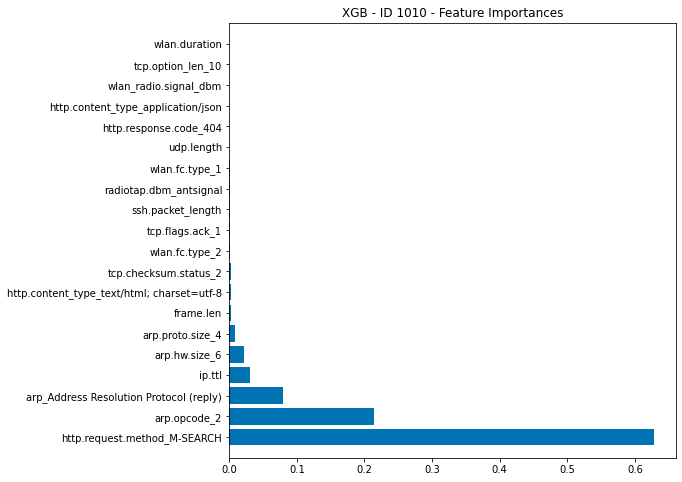
\includegraphics[width=\textwidth]{Appendices/Images/XGB/xgb_1010_fi.png}
%\label{fig:xgb_optimised_fi}
%\end{figure}
%
%\clearpage
%\begin{table}[hp]
%  \centering
%  \caption{Optimised XGBoost Classification Report}
%  \label{tab:optimised_xgboost}
%    \begin{tabular}{lcccc}
%    \toprule
%    Class & Precision & Recall & F1-Score & Support \\
%    \midrule
%    Botnet & 0.96 & {\color{red}\bfseries 0.75} & {\color{red}\bfseries 0.84} & 17060 \\
%    Malware & {\color{red}\bfseries 0.89} & 0.82 & 0.85 & 39476 \\
%    Normal & 1.00 & 1.00 & 1.00 & 4572206 \\
%    SQL Injection & 0.94 & 0.89 & 0.91 & 789 \\
%    SSDP & 1.00 & 1.00 & 1.00 & 1649955 \\
%    SSH & 0.92 & 0.78 & 0.85 & 3565 \\
%    Website Spoofing & 0.99 & 0.97 & 0.98 & 121533 \\
%    \midrule
%    Accuracy & & & 1.00 & 6404584 \\
%    Macro Avg & 0.96 & 0.89 & 0.92 & 6404584 \\
%    Weighted Avg & 1.00 & 1.00 & 1.00 & 6404584 \\
%    \bottomrule
%    \end{tabular}
%\end{table}
%
%\begin{figure}[H]
%\centering
%\caption{Optimised XGBoost Model CM}
%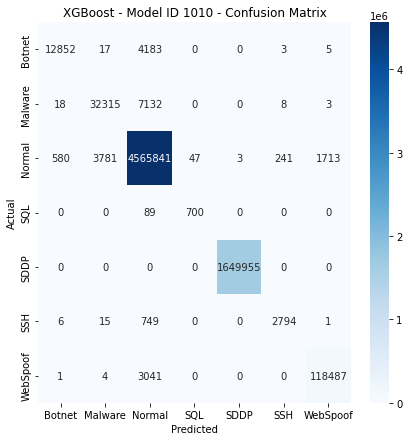
\includegraphics[width=0.9\textwidth]{Appendices/Images/XGB/xgb_1010_cm.png}
%\label{fig:xgb_optimised_cm}
%\end{figure}
